%%%%%%%%%%%%%%%%%%%%%%%%%%%%%%%%%%%%%%%%%%%%%%%%%%%%%%%%%%%
\subsection{Synthetic data generation}
%%%%%%%%%%%%%%%%%%%%%%%%%%%%%%%%%%%%%%%%%%%%%%%%%%%%%%%%%%%
%
%
\begin{frame}[t, negative]
	\subsectionpage
\end{frame}
%
%
\begin{lhframe}[rhgraphic={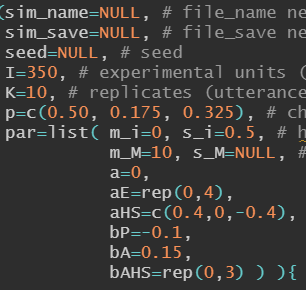
\includegraphics[scale=0.7]{sim_code1.png}}]
	{Idealized data\footnote{more details in file: \textcolor{blue}{\texttt{1\_2\_E\_sim\_fun.R} }}}
	
	Simulation data can serve as \cite{Kruschke_2014, McElreath_2020},
	\begin{enumerate}
		%
		\item A place where to test your model, on multiple purposes,
		%
		\begin{itemize}
			\item parameter recovery
			\item power
		\end{itemize}
		%
		\item A (possible) reflection of a population, 
		%
		\begin{itemize}
			\item children's group proportion \cite{DeRaeve_2016}
		\end{itemize}
		%
		\item A (possible) reflection of a hypothesis,
		%
		\begin{itemize}
			\item size of effects \alert{(no previous information)}
		\end{itemize}
		%
	\end{enumerate}
	%
\end{lhframe}
%
%
\begin{lhframe}[rhgraphic={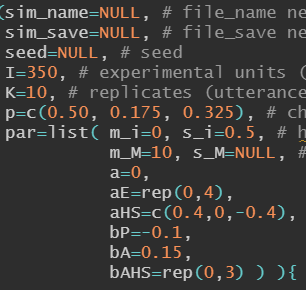
\includegraphics[scale=0.7]{sim_code1.png}}]
	{Idealized data}
	
	About the size of the effects \\
	\alert{(in logits, no previous info)},
	%
	\begin{enumerate}
		%
		\item $aE=-0.1$, assumes $E$ ordered by severity \alert{(it might not be possible)},
		%
		\item $aHS=-0.4$, assumes $0.4$ difference between $NH$ children and $HI/CI$,
		%
		\item $bP=-0.1$, assumes decrease of SI per $PTA$ unit \\
		($+10 \; PTA$ units $\Rightarrow -1$ logit),
		%
		\item $bA=-0.15$, assumes decrease of SI per $A$ unit, beyond the minimum \\
		($+10 \; A$ units $\Rightarrow +1.5$ logits),
		%
	\end{enumerate}
	%
\end{lhframe}
%
%
\begin{lhframe}[rhgraphic={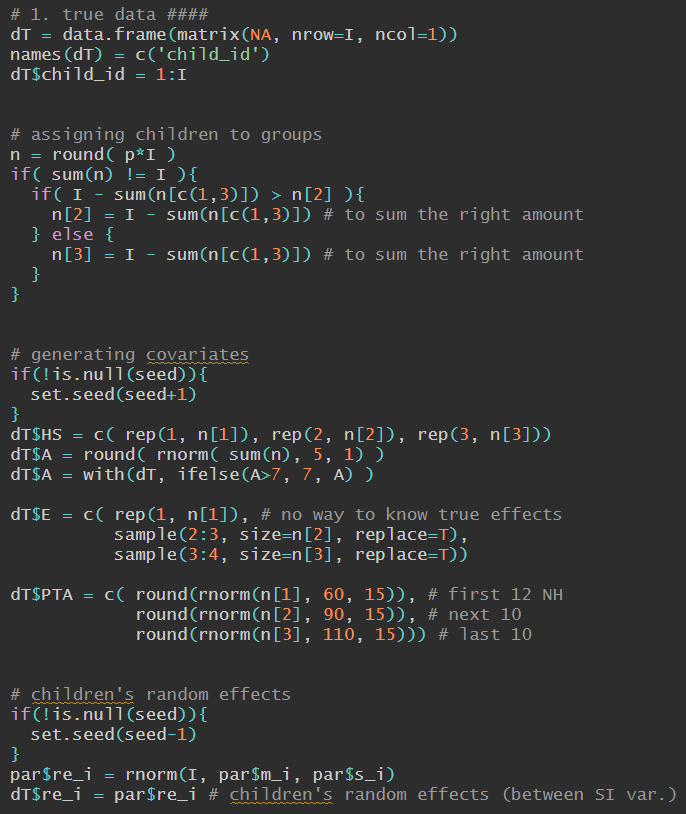
\includegraphics[scale=0.48]{sim_code2.png}}]
	{Idealized data}
	
	\begin{enumerate}
		%
		\item variables are generated in a random fashion 
		\item random effects define the between SI variability
		%
	\end{enumerate}
	%
\end{lhframe}
%
%
\begin{lhframe}[rhgraphic={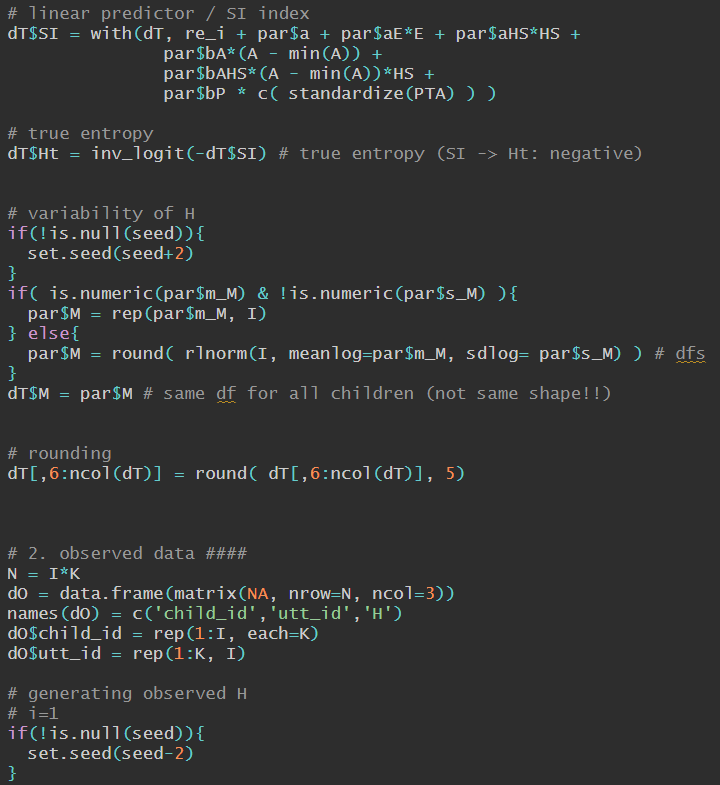
\includegraphics[scale=0.48]{sim_code3.png}}]
	{Idealized data}
	
	\begin{enumerate}
		%
		\item we use \textcolor{blue}{second form} of the probabilistic model
		\item ``true' entropy ($Ht$) is inversely related to $SI$
		\item we simulate measurement error through $M$ from $BetaProp()$ distribution (as previously shown).
		%
	\end{enumerate}
	%
\end{lhframe}
%
%
\begin{lhframe}[rhgraphic={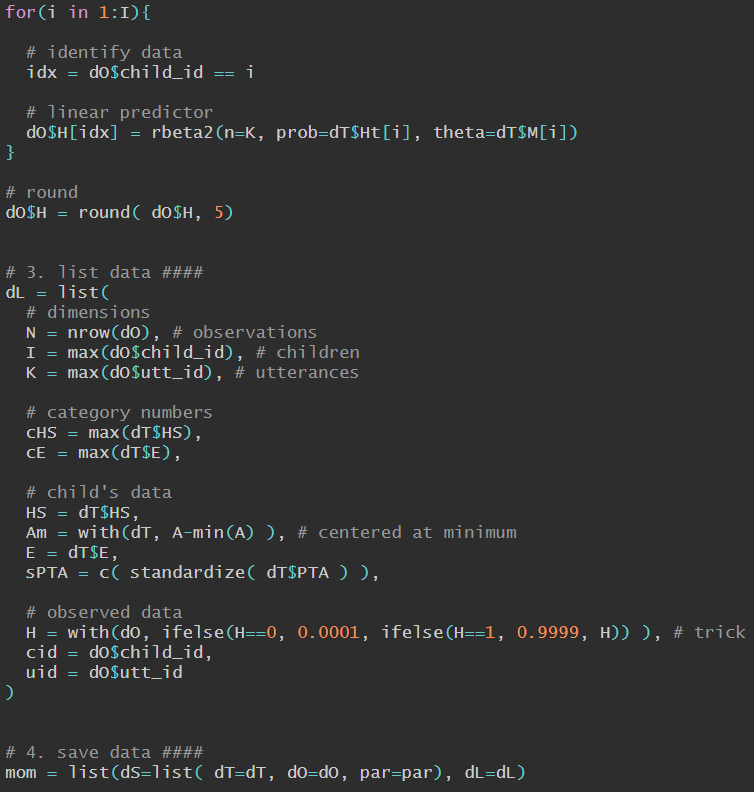
\includegraphics[scale=0.48]{sim_code4.png}}]
	{Idealized data}
	
	\begin{enumerate}
		%
		\item we simulate replicate measures of entropy ($H$)
		\item we storage all relevant parameters and data
		%
	\end{enumerate}
	%
\end{lhframe}
%
%
\begin{lhframe}[rhgraphic={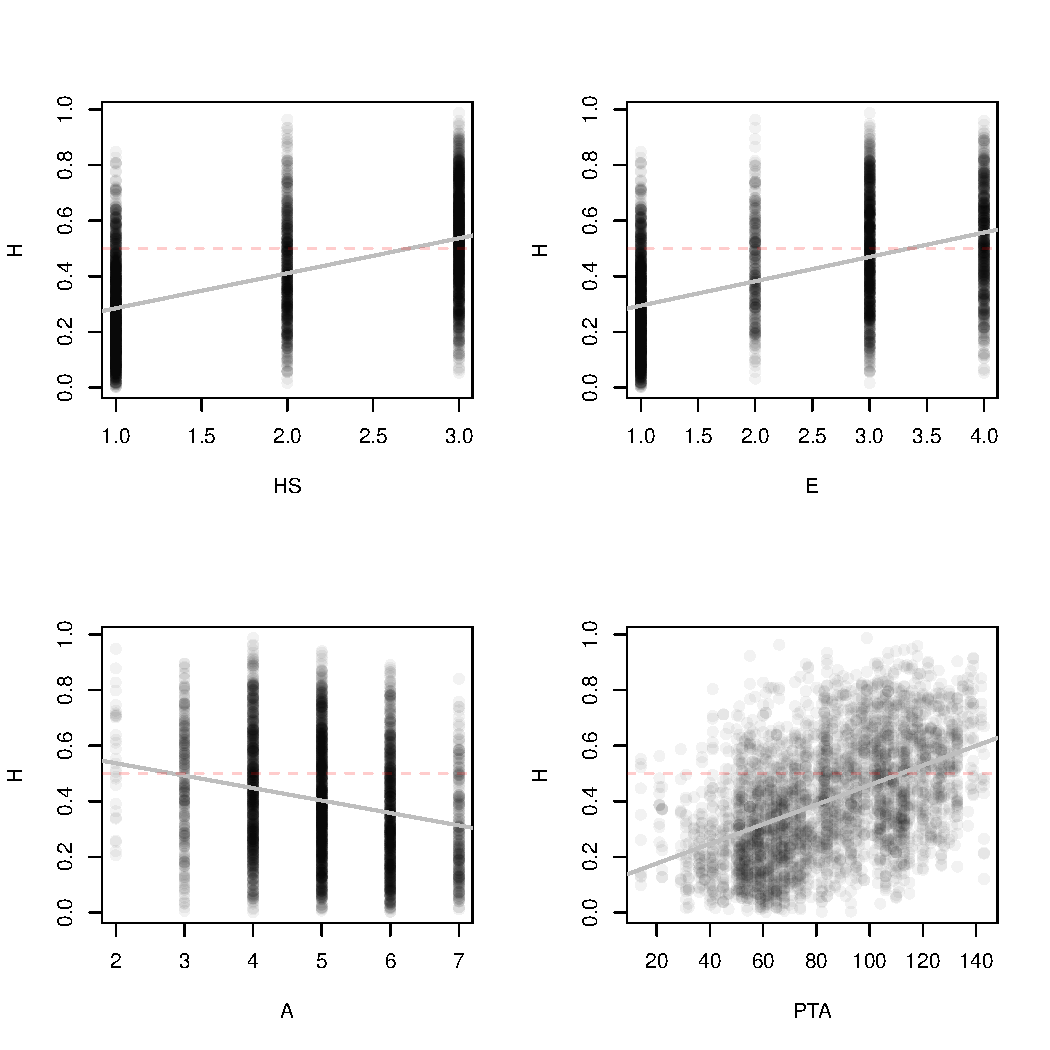
\includegraphics[scale=0.45]{data_example.pdf}}]
	{Example}
	
	notice we can simulate any desired relationship, or lack of thereof.
	%
\end{lhframe}
%
%